\section{METHODOLOGY}

\subsection{Overview of the Approach}

This study builds an agent-based model of RSSI management on sugarcane and uses it to compare four control strategies under sustained use: no control, chemical control, biological control, and a hybrid of the two. The model is exploratory. It is meant to show how the strategies rank under stated assumptions and how sensitive that ranking is to the assumptions that no source supports. It is not meant to predict infestation in any particular Negros field.

The work proceeds in three stages. Pre-modelling consists of the systematic review in the Review of Literature, the collection of data from the SRA and interviews, and the extraction of parameters with an explicit record of what the data cannot support. Model development consists of the conceptual model, its formal description, and its implementation in the GAMA platform \citep{Taillandier2019}. Verification and scenario exploration consist of code checks, the strategy experiments, and a hindcast against the SRA record of the outbreak. GAMA was chosen because grid and raster environments are the commonest representation in the reviewed models, GAMA handles them natively together with GIS layers, and no reviewed study used it.

\subsection{Conceptual Model}

The conceptual model was set out with the PARDI method (Problem, Actors, Resources, Dynamics, Interactions), which builds on the ARDI method of \citet{Etienne2011}. The problem is to determine which control strategy best manages RSSI on sugarcane over sustained use. The boundaries are kept narrow: RSSI on sugarcane only, the cane landscape of Negros Island, daily time steps over three crop years after the first infestation, and a relative comparison between strategies as the output. Resistance evolution at the genotype level and re-invasion from outside the island are out of scope. Resistance to chemicals enters only as a decline in chemical efficacy with repeated use, stated as an assumption.

Three actors matter in the system. Farmers observe infestation and choose a control action. Government bodies (the SRA, the Department of Agriculture, and local government units) fund and deliver control \citep{ChiniMandi2026,Partlow2026}, which the model represents through the hybrid strategy rather than as an agent. Mills and the sugar market set the prices that turn cane into income. The model leaves money out. No source gives a verifiable control cost per hectare, and revenue would be a constant multiple of cane, so the model reports applications by type in place of cost.

\begin{figure}[!htbp]
\begin{center}
	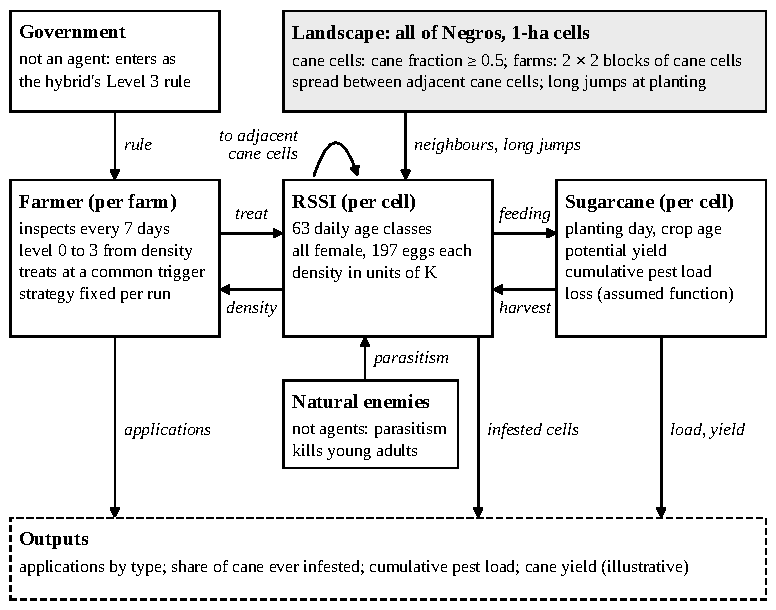
\includegraphics[width=\textwidth]{figures/fig-conceptual}
	\caption{Conceptual model. Pest, crop, and farmer are represented explicitly. Natural enemies and government enter as rules, not agents. Spread runs from an infested cell to its adjacent cane cells (loop). Arrows to the outputs show where each output is computed. Long jumps occur at planting and at ratooning. Harvest removes 90\% of the pest in a cell, an assumed value. Climate is held out.}
	\label{fig:conceptual}
\end{center}
\end{figure}

\subsection{Model Description}

The model is described with the ODD+D protocol \citep{Muller2013}. This section gives the structure. The full description, including every submodel, is kept in the project repository (\texttt{docs/model-odd-d.md}).

\subsubsection{Entities, landscape, and scales}

The landscape covers all of Negros Island, both provinces, at 1-ha resolution (Table~\ref{table:landscape}, Figure~\ref{fig:landscape}). It is a grid of 1,327 by 2,224 cells of 100 m by 100 m in UTM zone 51N, of which 1,278,239 cells lie inside the boundaries of the island's 57 cities and municipalities \citep{OCHA2025}. Each cell carries its municipality and its cane fraction, the share of its 10-m pixels mapped as sugarcane in the global sugarcane map of \citet{DiTommaso2024}, which classifies sugarcane from GEDI lidar and Sentinel-2 imagery over 2019--2022. A cell is a cane cell if its cane fraction is at least 0.5, so that every cane cell is mostly cane. This rule gives 356,869 cane cells. The count is sensitive to the rule (see Limitations of the Method). A 1-ha cell aggregates 100 pixels of the 10-m map. Farm size is not resolved: about 84\% of Philippine sugarcane farmers hold less than 5 ha \citep{PCAARRDnd}, but the share below 1 ha is not reported. Only cane cells hold a crop and a pest. All other cells are inert, and neighbour spread runs only between adjacent cane cells. The grid has a Moore neighbourhood.

The mapped cane area is larger than the area SRA reports as planted. The map gives 351,987 ha of cane on Negros against 239,216 ha planted in crop year 2025--2026, a ratio of 1.47 \citep{SRA2026FOI}. The ratio is 1.36 in Negros Occidental and 1.99 in Negros Oriental. Shares in this study are therefore shares of mapped cane cells, not of planted area, and the hindcast compares hectares by counting one cane cell as 1 ha (see Hindcast).

Roads come from OpenStreetMap \citep{OSM2026}. Trunk, primary, and secondary roads were retained, and cane cells within 100 m of one are flagged as roadside. The roadside flag can raise the long-jump probability of a cell (see Spread). At baseline its multiplier is 1 and the daily roadside inoculation is 0, so roads have no effect on the runs reported here.

\begin{figure}[!htbp]
\begin{center}
	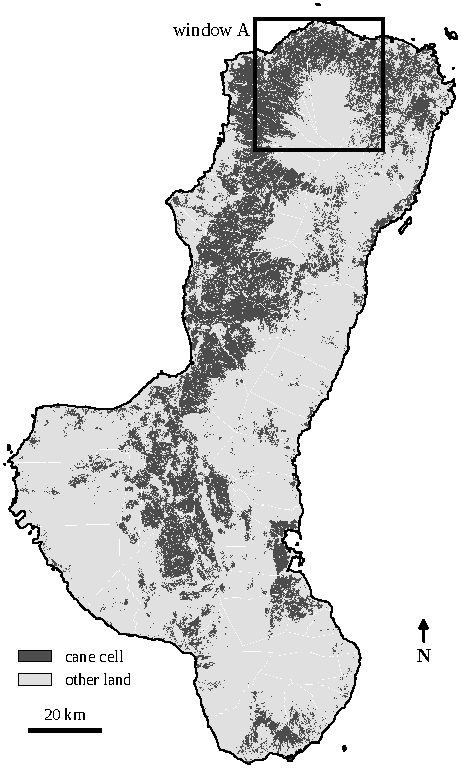
\includegraphics[width=0.55\textwidth]{figures/fig-landscape}
	\caption{Model landscape. Cane cells are 1-ha cells in which at least half the area is mapped as sugarcane in the 2019--2022 map of \citet{DiTommaso2024}. White lines are municipal boundaries \citep{OCHA2025}. The box marks window A (Cadiz City, Manapla, and the City of Victorias), used for the sensitivity analysis.}
	\label{fig:landscape}
\end{center}
\end{figure}

\begin{table}[!htbp]
\vspace{2ex}
\centering
\caption{Landscape inputs and their derived sizes. Counts are computed from the model input grids.}
\label{table:landscape}
\begin{tabular}{L{0.32\textwidth}L{0.6\textwidth}}
\hline\hline
Item & Value and source \\ \hline
Sugarcane & 10-m map, 2019--2022, CC BY 4.0 \citep{DiTommaso2024,DiTommaso2024data} \\
Municipal boundaries & COD-AB version 03, valid 13 February 2025 \citep{OCHA2025} \\
Roads & OpenStreetMap trunk, primary, secondary, downloaded 8 November 2026, ODbL \citep{OSM2026} \\
Grid & 1,327 $\times$ 2,224 cells of 1 ha, UTM zone 51N \\
Cells inside the 57 LGUs & 1,278,239 \\
Cane cells (cane fraction $\geq$ 0.5) & 356,869 \\
Farms (2 $\times$ 2 blocks of cane cells) & 112,713, of 1 to 4 ha \\
Sensitivity window A & Cadiz City, Manapla, City of Victorias: 32,335 cane cells, 10,611 farms \\ \hline\hline
\end{tabular}
\vspace{2ex}
\end{table}

One tick is one day. Day 0 is 1 October, the start of the planting window. The landscape runs free of the pest until the infestation is seeded on day 233, and a run then lasts 1,095 days, three crop years, to day 1,328 (see Initial conditions). A day is the finest scale at which any modelled process changes. The shortest developmental stages last 2 to 6 days, treatments are datable to a day, and egg incubation, the shortest life-history stage, would be skipped by a weekly step.

Each cane cell holds a crop and a pest population. The crop has a planting day, an age, a potential yield, a cumulative pest load, and a loss fraction. The pest is stage-structured and held as a density in each daily age class from 0 to 62 days, in units of the cell's carrying capacity $K$. A cohort representation was chosen over individual insects because each female lays about 197 eggs, and several generations of individuals would be too many agents to run. Farmers are agents. No farm-boundary data were found, so a farm is the set of cane cells in each 2 by 2 block of the grid, which gives 112,713 farms of 1 to 4 ha [assumption]. Each farmer has a level of infestation, a count of applications, and a current chemical efficacy. Natural enemies are not entities. Parasitism enters as a daily mortality term on young adults.

\subsubsection{Process schedule}

Each day the model executes nine steps in a fixed order, each over all cells before the next (Figure~\ref{fig:schedule}). The steps are calendar and crop (planting on a day drawn uniformly from the October to May window, harvest at crop age 365 days, then ratoon regrowth), pest ageing, reproduction, mortality from parasitism and from active treatments, spread, damage, farmer monitoring every 7 days, control, and recording of outputs. Control follows monitoring, so a farmer acts on the day an infestation is detected. To keep island-scale runs tractable, the code visits only the cells where something happens on a given day. This event-driven bookkeeping gave the same results as a full daily scan on window A with a fixed seed.

\begin{figure}[!htbp]
\begin{center}
	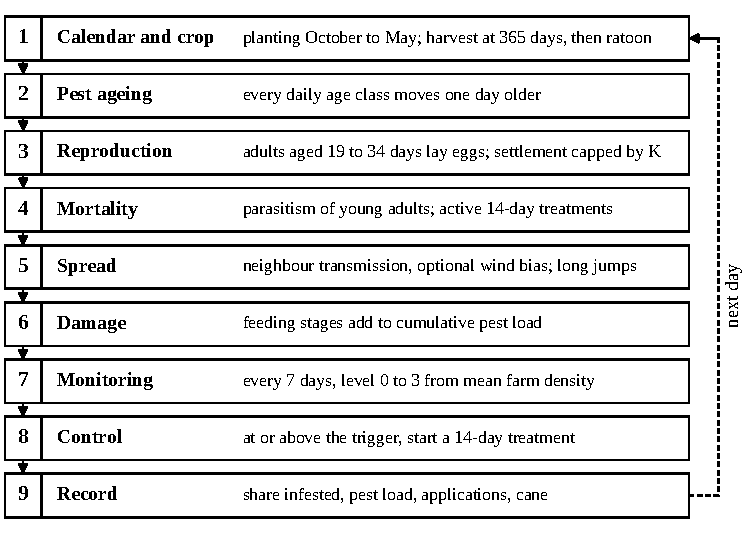
\includegraphics[width=0.85\textwidth]{figures/fig-schedule}
	\caption{Daily process schedule (one tick equals one day). Farmers monitor every 7 days, and each treatment acts for 14 days.}
	\label{fig:schedule}
\end{center}
\end{figure}

\subsubsection{Pest submodel}

Development is deterministic. Stage durations are fixed at the Philippine laboratory values at 27 to 29\,$^{\circ}$C \citep{Guerrero2026}, as one integer set chosen inside every reported range and summing to the reported 63-day cycle from egg to death: egg 2 days, three instars of 6, 6, and 5 days, then young, mature, and senescing adult stages of 13, 17, and 14 days (Figure~\ref{fig:lifecycle}). Reproduction is all-female. Females lay at adult ages 19 to 34 days, 197 eggs in total, taken as 12.31 eggs per day over 16 days. Settled recruits equal eggs multiplied by a settlement survival and by a density-dependent term, one minus the density of feeding stages over $K$. Settlement survival lumps egg, crawler, and settlement losses into one free parameter because no stage-specific field mortality has been measured. Climate is held out. Development runs at the single laboratory rate of \citet{Guerrero2026}.

\begin{figure}[!htbp]
\begin{center}
	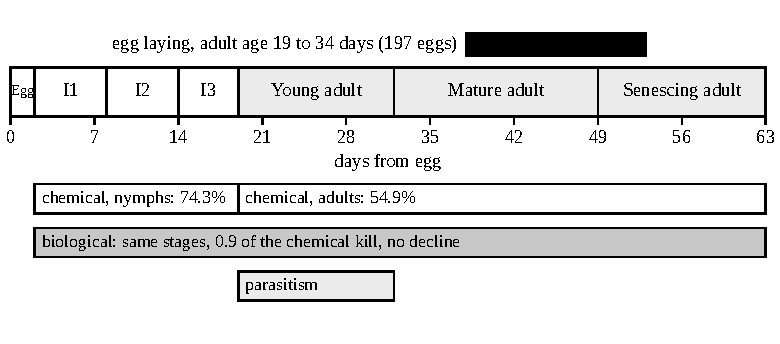
\includegraphics[width=\textwidth]{figures/fig-lifecycle}
	\caption{RSSI life cycle as coded, from egg to death in 63 days \citep{Guerrero2026}, and the stages each control acts on. Chemical kill fractions are medians of six compounds on first application \citep{SRAnd}, applied in the model over 14 days. Shaded stages are adults.}
	\label{fig:lifecycle}
\end{center}
\end{figure}

\subsubsection{Spread}

RSSI adults are fixed to the leaf and crawlers move only within the plant, so the model gives the insect no dispersal distance. An RSSI researcher interviewed for this study stated that between-field spread is driven by external factors and that no rate can be calculated (G.~A.~S. Burgonio, personal communication, 21 September 2026). The model therefore uses two mechanisms with swept, unsourced parameters. In neighbour transmission, a planted cane cell receives crawlers with probability $1-\exp(-\beta P)$, where $P$ is the summed density of its infested cane neighbours on the previous day and $\beta$ is a transmission rate. A wind bias can weight each neighbour by $\max(0, 1 + b\cos(\theta-\phi))$, where $\theta$ is the direction from the neighbour to the cell and $\phi$ is the direction the wind blows toward. The direction is set to the annual prevailing wind at Dumaguete, from the north-east \citep{PAGASAnd}, the only official 1991--2020 normals found for the island. The strength $b$ is 0 at baseline and is tested at 0.5 and 1. Long jumps stand for planting material and cane transport. At planting and at ratooning, a cell may be inoculated with a probability proportional to the share of cane cells currently infested, multiplied for roadside cells by the roadside factor. Both mechanisms are assumptions. They are the least parameterised part of the model, and the sensitivity analysis treats them accordingly.

\subsubsection{Damage}

Damage follows the structure of the closest sugarcane precedent \citep{Alves2026}, in which each pest removes a unit of the crop attribute per step. Each day the feeding stages (ages 2 to 62 days) add to the cell's cumulative pest load, in capacity-days (K-days). Loss is linear in the load accumulated by the current crop and capped at a maximum, with a saturating form available as a robustness check. The slope is set by an interpretable anchor: a cell held at capacity for a whole crop year loses 30\% of yield. No Philippine study has quantified RSSI yield loss \citep{Guerrero2024}, so this coupling is assumed. The provincial dashboard describes visible damage from moderate severity and possible yield loss at high severity \citep{PGNO2026}. This is consistent with loss that rises with pest density, but it gives no values. Two consequences follow and are stated here so that they are not mistaken for findings. Under linear damage, the strategy ranking by yield loss equals the ranking by cumulative pest load whatever the slope, so cumulative pest load and the share of cane ever infested are the primary outputs and cane yield is an illustrative rescaling. Sugar is cane multiplied by a constant recovery, so sugar cannot respond to the strategy and is not reported.

\subsubsection{Control and the farmer decision}

Farmers follow a fixed reactive rule. Every 7 days a farmer reads the mean pest density over its planted cells and assigns an infestation level from 0 to 3. The levels follow the provincial task force, which defines Levels 1 to 3 as 1 to 5, 6 to 10, and more than 10 insects per leaf \citep{PGNO2026}. The model holds density in units of the carrying capacity $K$, and no source gives $K$ in insects per leaf. The conversion therefore assumes 100 insects per leaf at capacity, chosen so that one insect per leaf equals the density at which a cell counts as infested (0.01\,$K$). This gives thresholds of 0.01, 0.06, and 0.11\,$K$ on the farm mean density. The conversion is swept at 50 and 200 insects per leaf, which doubles and halves the three thresholds together. Two differences from the survey remain. The task force counts insects on one leaf per farmlot, while the model uses the mean over a farm's planted cells. Whether these levels are the same scheme as any levels used by the SRA is not confirmed. A farmer acts when the level reaches a trigger, Level 1 at baseline, and the 14-day re-treatment interval has elapsed. One trigger applies to every strategy, so that the comparison reflects the control agent and not an earlier start for one of them. Under the biological strategy the agent is an entomopathogenic fungus. The province applies \emph{Metarhizium} and \emph{Beauveria} \citep{PGNO2026}, but the model's biological kill is set from \emph{Metarhizium} data only. Under the hybrid strategy the fungus is used at Levels 1 and 2 and a chemical at Level 3, following a press report that fungi target the lower levels while local governments lead on Level 3 \citep{Gomez2026}. That Level 3 action is chemical is an inference, as the source does not state it.

A treatment acts as a daily kill hazard on nymphs and adults for 14 days. Chemical and biological treatments share the same stages and time course. The 14-day chemical kill uses the median of six compounds on first application, 74.3\% on nymphs and 54.9\% on adults, from a National Crop Protection Center progress report summarised by the SRA \citep{SRAnd}. This is a single unreplicated report whose measurement interval is not stated. The biological kill is a fixed fraction of the chemical kill, 0.9 at baseline, bounded by the field ratio of \emph{Metarhizium} to malathion reductions \citep{Sallam2021} and by parity in a laboratory assay \citep{Buletin2026}. Chemical efficacy declines with repeated use on the same farm, halving after a set number of applications: no decline, 20 applications, or 10 applications in the main comparison, and 40, 80, and 160 applications in a follow-up test. These values are arbitrary and labelled as such. The biological agent does not decline at baseline. A test setting applies the same halving rule to the biological agent, with each agent's applications counted separately on a farm. The decline is a per-farm rule on efficacy and represents no resistance biology. The only Philippine repeat-application data show nymph efficacy falling and adult efficacy rising between first and second application \citep{SRAnd}. The modelled chemical strategy repeats one mode of action without rotation, which departs from the rotation of modes of action the SRA recommends \citep{SRAnd}.

\subsubsection{Initial conditions}

The outbreak is started from its first declared extent. The SRA declared an infestation on 22 May 2025, when RSSI had spread over 87 ha in Negros Occidental \citep{ManilaBulletin2025}. Day 0 of a run is 1 October 2024, so 22 May 2025 is day 233. The landscape is free of the pest until that day, by which time the cane planted from 1 October to 21 May is standing. On day 233 the model seeds 87 planted cane cells, 87 ha, each at a density of 0.05\,$K$ as third instars. The cells lie in the 11 local government units reported as affected four days later: the cities of Silay, Talisay, Victorias, Cadiz, Bago, and La Carlota, and the municipalities of E. B. Magalona, Manapla, Toboso, Murcia, and La Castellana \citep{Guadalquiver2025}. No source gives the area by unit, so the 87 cells are split equally across the units present in the landscape and placed at random within each unit's cane. On the island this is 7 cells in each of the 11 units, with the remaining 10 placed at random among them. On window A, which contains three of the 11 units, it is 29 cells in each. The equal split, the placement within a unit, and the seed density are assumptions. The seed size is not swept.

\subsection{Parameterisation and Data}

Every parameter carries a source and a status: real (a Philippine or Negros source for that quantity), real with a stated conversion, analogue (another region, laboratory to field, or a related quantity), or assumption (no source). Table~\ref{table:params} gives the parameters that drive the model. The full table of 50 rows, with page-level sources and swept ranges, is kept in the project repository. Ranges described as arbitrary span qualitatively different behaviour and are not claimed to bound the truth.

{\small\singlespacing
\begin{longtable}{L{0.25\textwidth}L{0.15\textwidth}L{0.15\textwidth}L{0.2\textwidth}L{0.11\textwidth}}
\caption{Main parameters (compressed from the full parameter table).}\label{table:params} \\
\hline\hline
Parameter & Baseline & Swept range & Source & Status \\ \hline
\endfirsthead
\multicolumn{5}{l}{\emph{Table~\ref{table:params}, continued.}} \\
\hline\hline
Parameter & Baseline & Swept range & Source & Status \\ \hline
\endhead
\hline\hline
\endlastfoot
Stage durations & 2, 6, 6, 5, 13, 17, 14 d (63 d) & fixed & \citet{Guerrero2026} & real \\
Fecundity, laying window & 197 eggs, adult age 19--34 d & fixed & \citet{Guerrero2026} & real \\
Settlement survival & 0.05 & 0.01--0.10 & none & assumption \\
Neighbour transmission $\beta$ & 0.1 per $K$ per day & $\times$0.25, $\times$4 & none & assumption \\
Long-jump probability & 0.05 & 0, 0.2 & none & assumption \\
Wind bias $b$ (direction from NE) & 0 & 0.5, 1 & \citet{PAGASAnd} for direction & assumption \\
Seed, day 233 (22 May 2025) & 87 cells at 0.05\,$K$ & not swept & \citet{ManilaBulletin2025} for area; split and density assumed & real, converted \\
Chemical 14-d kill, nymphs; adults & 0.743; 0.549 & not swept & \citet{SRAnd} & real, converted \\
Biological to chemical efficacy ratio & 0.9 & 0.8, 1.0 & \citet{Sallam2021}, \citet{Buletin2026} & analogue \\
Chemical efficacy decline & none & 160, 80, 40, 20, 10 applications to half & none & assumption \\
Biological efficacy decline & none & 80, 20 applications to half (test only) & none & assumption \\
Parasitism of young adults & 0.3485 & 0, 0.668 & \citet{Guerrero2024}, \citet{Navasero2023} (Luzon) & analogue \\
Level thresholds & 0.01, 0.06, 0.11\,$K$ & $\times$0.5, $\times$2 & \citet{PGNO2026}: 1, 6, 11 insects per leaf & real, converted \\
Insects per leaf at $K$ & 100 & 200, 50 & none & assumption \\
Trigger level & 1 & 2, 3 & none & assumption \\
Re-treatment interval & 14 d & 7, 28 d & \citet{SRAnd} & analogue \\
Cane fraction for a cane cell & 0.5 & not swept & none & assumption \\
Potential yield & 61.64 t/ha & not swept & \citet{SRA2026FOI}, mean 2020--2025 & real, converted \\
Loss at a full season at capacity; maximum loss & 0.3; 1.0 & 0.1--0.5; 0.5, 1.0 & none & assumption \\
\end{longtable}
}

Data for the model came from five places. The laboratory biology comes from published Philippine work. Crop baselines (area and cane yield by Negros mill district for crop years 2020--2021 to 2025--2026, and sugar recovery for 2025--2026) came from the SRA reply to a freedom-of-\allowbreak information request filed on 30 September 2026 \citep{SRA2026FOI}. The same reply gave one snapshot of RSSI-affected area by municipality, dated 2 October 2026, without infestation levels or a map. It did not include Negros parasitism rates, cost per hectare, or the SRA weather studies. The provincial monitoring dashboard gives the per-leaf definitions of the infestation levels and a dated survey of severity across Negros Occidental \citep{PGNO2026}. Its farmlot counts measure survey effort, not affected area, so they are not compared with the SRA hectares. The landscape layers came from the open datasets in Table~\ref{table:landscape}. The missing items are handled as swept assumptions, and the outputs are framed as relative comparisons, with the unsupported quantities deferred to later work.

\subsection{Implementation}

The model is implemented in GAMA \citep{Taillandier2019}. The code was audited against the ODD+D on 4 November 2026. Ten mismatches were found and nine were fixed, and the audited model compiles without errors. On 8 November the landscape was moved from a 50 by 50 stylised grid to window A and then to the whole island, and on 13 November the random start and the earlier arbitrary level thresholds were replaced by the seeded start and the provincial levels. Strategies are a switch, and every unsourced assumption is exposed as a parameter, so that none is hard-coded.

All reported runs were made with GAMA 2026.11.0 in headless mode on a 16 GB laptop, between 14 and 16 November 2026. Each GAMA process held one simulation at a time, because a single island simulation needs most of the available memory. Every batch finished with exit code 0. Each run writes one row of outputs at its last day. Selected island runs also write a weekly series and, on day 731, the number of cane cells ever infested in each municipality.

\subsection{Verification, Experiments, and Hindcast}

\subsubsection{Verification}

Two checks test the code before any batch is read. In the life-table check, a single cohort in one cell with no recruitment must disappear on day 63 and lay 197 eggs per female multiplied by one minus the parasitism rate. The expected values are 197.00, 128.35, and 65.40 eggs per female at parasitism of 0, 0.3485, and 0.668, with 1.0, 0.6515, and 0.332 of the cohort remaining after the young-adult stage. In the no-pest check, a landscape without pests must show no infestation, no treatment, and the input potential yield at harvest. Both checks passed on the island landscape on 11 November 2026: the cohort runs gave the expected values to rounding, and the no-pest run gave no infestation, no applications, and 61.64 t/ha at harvest. The life-table values also match a separate replica of the same equations written in Python. These checks were made before the seeded start and the new level thresholds were added on 13 November and have not been repeated since. Neither change touches the life table or the crop bookkeeping that the checks test. Two properties of the seeded runs serve as further checks. With the biological efficacy ratio set to 1.0, the biological strategy is the same process as chemical control without decline, and the two gave loads within replicate spread of each other (ratio 0.96). The damage form does not act on the pest, and runs with the saturating form gave pest loads within replicate spread of the linear runs.

\subsubsection{Experiments}

The experiments run at two scales. The whole island carries the main comparison and the hindcast. Window A, the cane landscape of Cadiz City, Manapla, and the City of Victorias in northern Negros Occidental (32,335 cane cells, 10,611 farms), carries the main comparison again and every test that needs many runs, at a scale where a run takes minutes. All runs use the seeded start and last 1,095 days after seeding unless stated.

The main comparison covers the four strategies. Chemical efficacy decline matters only where chemicals are applied, so chemical control is run at three decline settings (none, and halving every 20 and every 10 applications). No control and biological control are run once each. The hybrid is run at decline 20 on the island and at all three settings on window A. This gives six configurations on the island and eight on window A. The primary outputs are cumulative pest load (K-days summed over cells) and the share of cane cells ever infested. The share infested at the end, applications by type, and cane yield per harvested hectare are secondary. Applications are counted as farm-level treatment events. Cane yield follows from the assumed damage slope and is reported only as an illustration.

Window A carries six further sets of runs (Table~\ref{table:design}). The sensitivity analysis follows the one-at-a-time design of \citet{Alves2026}. Each of nine unsourced assumptions is moved to a low and a high value, with chemical decline fixed at 20 applications: settlement survival, neighbour transmission, long-jump probability, parasitism, the biological efficacy ratio, the level thresholds, the trigger level, the re-treatment interval, and wind bias. This gives 18 cases plus the baseline for the four strategies. The question for each case is whether the strategy ranking changes or only its magnitudes. A wind-direction check compares wind from the north-east and from the south-west at full bias. A damage-form check repeats the baseline with the saturating form. A decline test runs chemical control with efficacy halving every 40, 80, and 160 applications, to locate the rate at which chemical control matches the biological and hybrid strategies. A hybrid test runs the chemical, biological, and hybrid strategies, with no chemical decline, under the two sensitivity settings in which farms reach Level 3 (treating only at Level 3, and re-treating every 28 days). A biological-decline test applies the halving rule to the biological agent, every 20 and every 80 applications, for the biological and hybrid strategies. Harvest removal of the pest, the seed size, and the roadside parameters are held at baseline and not swept. Damage slope and maximum loss are not swept, because damage does not act on the pest and so cannot change the ranking by pest load.

\begin{table}[!htbp]
\vspace{2ex}
\centering
\small
\caption{Run design. All runs use the seeded start. Counts are rows in the output files.}
\label{table:design}
\begin{tabular}{L{0.3\textwidth}L{0.42\textwidth}rr}
\hline\hline
Set & Configurations & Runs each & Runs \\ \hline
\multicolumn{4}{l}{\emph{Island}} \\
Main comparison & none; chemical (no decline, 20, 10); biological; hybrid (20) & 2 (none: 3) & 13 \\
Hindcast probes, no control, 735 days & transmission $\times$2.5, $\times$3, $\times$4; long jump 0.2; transmission $\times$4 with long jump 0.2 & 1 & 5 \\
\multicolumn{4}{l}{\emph{Window A}} \\
Main comparison & none; chemical (3); biological; hybrid (3) & 2 & 16 \\
Sensitivity & 19 cases $\times$ 4 strategies & 1 & 76 \\
Wind direction & 2 directions $\times$ 4 strategies & 2 & 16 \\
Saturating damage & 4 strategies & 2 & 8 \\
Chemical decline & 40, 80, 160 applications & 2 & 6 \\
Hybrid test & 2 settings $\times$ 3 strategies & 2 & 12 \\
Biological decline & 2 rates $\times$ 2 strategies & 2 & 8 \\ \hline
Total & & & 160 \\ \hline\hline
\end{tabular}
\vspace{2ex}
\end{table}

\subsubsection{Replicates and the reading of differences}

Following the adviser's guidance to use as few runs as acceptable, each configuration has two runs (three for island no control), and each sensitivity cell has one. Two runs cannot estimate the variance of a single configuration, so run-to-run noise is estimated by pooling. Window A has 20 pairs of runs that share a configuration, and the standard deviation of the log of the load is pooled within strategy across these pairs. From the pooled values, the means of two configurations with two runs each are read as different only if their ratio exceeds a noise band of two standard errors, which is 1.07 to 1.17 depending on the strategies compared. Two single runs are read as tied when their ratio falls inside the wider band for single runs, 1.25 for biological against hybrid. Because damage does not act on the pest, and because the hybrid applied no chemical at baseline, some configurations are replicates of the same process. They are pooled where a comparison needs more than two runs. No significance test is made, and the sensitivity screen, at one run per cell, shows whether a ranking flips and not how firmly it holds.

\subsubsection{Hindcast}

The model cannot be calibrated. No Negros time series of infestation by level was found \citep{SRA2026FOI,PGNO2026}, no Philippine study has measured damage \citep{Guerrero2024}, no spread rate can be calculated (G.~A.~S. Burgonio, personal communication, 21 September 2026), and the free parameters are swept assumptions. The seeded start does allow a hindcast: the model is started from the declared extent of 22 May 2025 and read on day 731, 2 October 2026, the date of the one verified island-wide figure, 72,103 ha of validated RSSI-affected area \citep{SRA2026FOI}. Three comparisons are made.

The first is area. The number of cane cells ever infested by day 731, at 1 ha each, is compared with the validated area, for the hybrid baseline and for no control. No control is the model's upper bound for that date, whereas the observed area was under treatment, with about 53\% of it treated by 2 October \citep{SRA2026FOI}. Where the baseline falls short, five further no-control runs raise the neighbour transmission rate or the long-jump probability to find what rate would reach the validated area. A rate found this way is one parameter tuned to one number with control ignored. It is reported as tuned to one point and is not used in the strategy comparison, which keeps the baseline values throughout.

The second is the pattern by municipality. The share of each municipality's cane cells ever infested by day 731 is compared with the SRA validated area as a share of its cane cells, by Spearman rank correlation over the 56 municipalities with cane and an SRA record, and again over the 45 that were not seeded. The seeded units start ahead by construction, so the second figure is the test of spread.

The third is the trajectory. The weekly series of area ever infested is set beside the dated official figures that could be verified: 87 ha on 22 May 2025 \citep{ManilaBulletin2025}, 4,923 ha on Negros Island on 11 September 2025 \citep{MojicaSevilla2025}, and 72,103 ha on 2 October 2026 \citep{SRA2026FOI}. These figures differ in metric (affected, infested, validated) and in scope, and the early ones partly reflect detection catching up, so they are read as a weak check on dates not used for tuning.

One further pattern uses the provincial survey. Among farms with RSSI in the hybrid run, the split across Levels 1 to 3 over 22 July to 8 November 2026 is compared with the split among surveyed farmlots where RSSI was found, 53\%, 31\%, and 16\% \citep{PGNO2026}. The survey's coverage grew over that period and its farmlots are not a sample of all farms, so this is a face-validation pattern only.

\subsection{Limitations of the Method}

The following limitations bound what the model can support. They are dated where they depend on data that may change.

\begin{enumerate}
	\item \emph{Dated and incomplete land cover.} The cane map covers 2019--2022, before RSSI reached Negros, and its cane area exceeds the 2025--2026 planted area by 47\% overall and by 99\% in Negros Oriental \citep{DiTommaso2024,SRA2026FOI}. The 0.5 cane-fraction rule is an assumption. A rule of 0.3 or 0.7 would give 436,480 or 268,793 cane cells instead of 356,869 [computed, not run]. The rule also drops fragmented cane. In San Jose, Negros Oriental, the map shows 106 ha of cane but the model keeps only 43 cane cells, fewer than the 95.13 ha SRA validated there as affected \citep{SRA2026FOI}. Municipal boundaries are indicative and still code the two provinces under their former regions \citep{OCHA2025}. Farm boundaries are assumed.
	\item \emph{Few replicates.} Configurations have two runs and sensitivity cells one, so differences are read only against pooled noise bands, not by a statistical test, and rare outcomes are not captured. The random seed of each run was not recorded correctly in the output files (every row reads 1.0), so individual runs cannot yet be reproduced exactly.
	\item \emph{Sensitivity on window A only.} The one-at-a-time analysis runs on three neighbouring, cane-dense municipalities in northern Negros Occidental. A ranking that holds there may not hold for the fragmented cane of Negros Oriental or for the island as a whole, where spread has further to travel.
	\item \emph{Seeding by assumption.} The 87 seeded cells are split equally across the 11 units first reported as affected and placed at random within them, because no area by unit or location was published \citep{ManilaBulletin2025,Guadalquiver2025}. The model therefore cannot reproduce where the outbreak is, and its spatial outputs say nothing about where the pest will spread next.
	\item \emph{The hindcast is not validation.} It compares the model with one verified administrative figure, taken while the area was under treatment, and with one dated survey snapshot. At best it shows whether baseline spread is of the right order. It cannot test the spread parameters.
	\item \emph{Assumed couplings and single sources.} Spread, damage, settlement survival, efficacy decline, the level thresholds in units of $K$, and the biological efficacy ratio have no direct source. The chemical kill rests on one unreplicated progress report \citep{SRAnd}, and parasitism rates come from Luzon \citep{Guerrero2024}. Climate is held out, so the model cannot say whether hot and dry conditions favour the pest. Farmers are homogeneous, follow one rule, and inspect without error.
\end{enumerate}

Outputs are therefore read as relative comparisons between strategies under stated assumptions.
